\documentclass[12pt,a4paper]{article}
\usepackage[english]{babel}
\usepackage{mathptmx, amsmath}
\usepackage[utf8x]{inputenc}

\usepackage{anysize}
\marginsize{30mm}{30mm}{15mm}{15mm}	
 
\usepackage{epsfig}	

\usepackage{fancyhdr}
\pagestyle{fancy}
\fancyhead{}
\fancyhead[L]{\small{BMLFlowVisualizer documentation}}
\fancyhead[C]{\small{}}
\renewcommand{\headrulewidth}{0pt}

\usepackage{wrapfig}
\usepackage{color}
\usepackage[usenames,dvipsnames]{xcolor}
\usepackage{hyperref}


\begin{document}

\title{\bf{AsapBMLFlowVisualisation}}
\date{\today}
\author{Jan Pöppel \\[3mm]
{\tt jpoeppel@techfak.uni-bielefeld.de}}
\maketitle\thispagestyle{empty}

\section*{Quickstart}

From \textbf{AsapRealizerDemo/java/resource/} run \\
\textbf{go.bmlflowvisualizer} 
~\\~\\
Spread needs to be running for the BMLFlowVisualizer to work.
Basic information about the program and it's functionality can be found under the 
Info menu (Menu $\rightarrow$ Info).

\tableofcontents

\clearpage
\section{Overview}

The BMLFlowVisualizer is a tool designed to visualise the bml flow in a running Asap environment. It allows the user to see what kind of bml blocks are send over 
ipaaca at what time. The bml blocks can also be inspected to view their messages. 
Furthermore the user gets information about the current scheduling state of already received bml blocks. 

\section{Installation}

The BMLFlowVisualizer comes with a \textit{build.xml} allowing the use of \textit{ant}. This has so far however only been tested within the working environment of the Sociable Agents Group of the university of Bielefeld and some commands might not work in different environments.

\section{Functionality}

This tool is supposed to make it easier to understand and debug the bml flow in an Asap environment. To that end, the bml blocks are shown in their temporal context as well
as in the context of their connections (see section \ref{sec:mainWin} for details). More detailed information about a certain bml block can be browsed by opening
the BML Information Window (see section \ref{sec:bmlinfo}) by double clicking a block in any of the visualisations. Furthermore it is possible to search for a specific
block using the search window (\ref{sec:search}). A recorded session can also be stored and loaded at a later time using the \textit{Save} and \textit{Load} options, 
provided by the menu or their respective shortcuts $CTRL+S$ and $CTRL+L$. A short summary about the different colours (see section \ref{sec:colours} for more details) 
and the basic functionality of the tool can be viewed using the Information Window, accessible using the menu button \textit{Info} or the shortcut $CTRL+I$.

\section{Details}

This section gives more detailed information about the different windows and the meaning behind the block colours.

\subsection{Main Window} \label{sec:mainWin}
Figure \ref{fig:overview} shows the main window of the BMLFlowVisualizer. The left half of the window visualises the history of the current Asap session, while the right
half visualises more detailed information about the current time. The red line on the left (as well as the number in the textbox below) 
indicates the current time, which detailed visualisation can be seen on the right half. 

The history section is basically separated into 3 subsections. The top subsection visualises the blocks in their planning phase (submitted and in preparation).
The second subsection visualises the blocks in their scheduling phase (pending and lurking). The last subsection shows the blocks in their execution phase 
(e.g. in\_exec and done). All blocks should go through all three phases and be represented in each of them. The width of each block visualises the time 
the block has spend in its three phases (planning, scheduling and execution). 

The detailed section consist of two panels. The top panel visualises the bml blocks that are currently being planned, while the lower one visualises the blocks that are 
currently being scheduled and playing. It also shows their relative connection to each other. A dotted line between two blocks means that they have an \glqq append\grqq connection
while a complete line means that they have a \glqq chunk\grqq connection. In the detailed section the block width has no special meaning.

The main window also provides a few control options: The first from the left in figure \ref{fig:overview} allows to set the current time. The time can be set using the textbox and the button \textit{Jump to time}. 

The slider allows to zoom in and out of the history panels. 

The \textit{Play} button \glqq plays\grqq back the recorded session starting from the current time all the way to the end. When playing the button will toggle to \textit{Pause} which stops the playback. 

The last button \textit{Go to End} moves the current time to the last recorded timestep.

The checkbox \textit{Update on feedback only} controls the way the bml flow is recorded. The default setting starts recording when the first bml message is received and stops when no new message was received for at least fife seconds. During this time the visualisation is updated every 100ms. When checked the visualisation will only be updated when a new bml message is received, resulting in a lower consumption of resources at the cost of jumping visual updates.

\begin{figure}[!htb]
\centering
 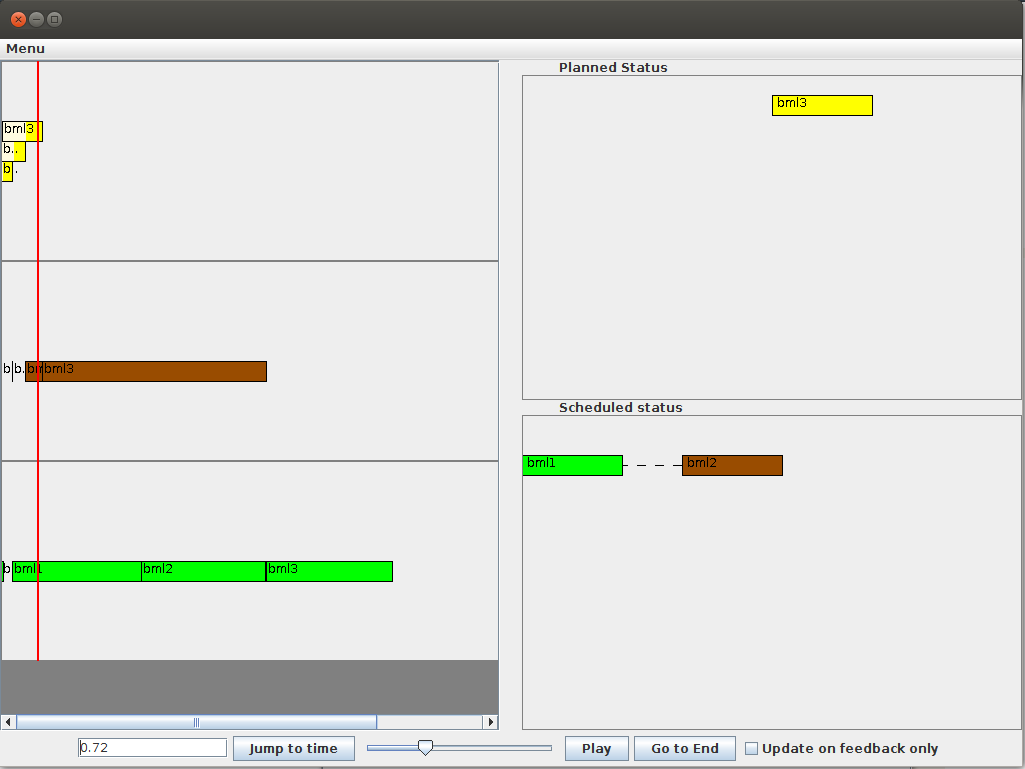
\includegraphics[width=\textwidth]{images/bmlFlowOverview.png}
 \caption{Main window of the BMLFlowVisualizer. The left half visualises the time history of the current session, while the right half shows more detailed information
 about the current timestep. The red line on the left symbolises the current time.}
 \label{fig:overview}
\end{figure}

\clearpage
\subsection{Search Window} \label{sec:search}

Figure \ref{fig:search} shows the search window that can be accessed using the menu or the shortcut $CTRL+F$. It allows to find a specific bml block since it lists all received blocks in a sortable table. The table can be sorted by any column by clicking at the column headers. A double click on any block row opens the block information window (see section \ref{sec:bmlinfo}) about that block.

Furthermore the textfield at the bottom allows to search for a specific bml block by it's id. The id does not need to be known completely since the search will toggle through all bml blocks that have a matching prefix when the \textit{Search} button is pressed. The row of the currently found bml block is highlighted as can be seen in the figure.

\begin{figure}[!htb]
\centering
 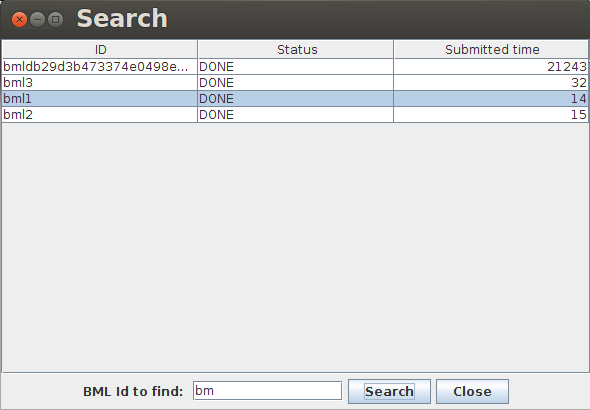
\includegraphics[width=\textwidth]{images/bmlFlowSearch.png}
 \caption{Search window of the BMLFlowVisualizer. Shows all received bml blocks with their current status and the time of their submission.}
 \label{fig:search}
\end{figure}

\subsection{BML Information Window} \label{sec:bmlinfo}

Figure \ref{fig:info} shows the information window for the block with the id bml1. The three columns show all information about the block. The first column shows the behaviours this block contains. The middle column lists all the messages the were received related to this bml block. A double click on any of the messages opens up a popup showing the actual xml of the message as can be seen in the second window in figure \ref{fig:info}. The last column shows the states the block has been in so far. Highlighted in yellow is the current state and the last received message (according to the current time selected in the main window). By selecting either a message or a state and using the \textit{Jump to selected time} buttons will set the current time in the main window to the time of the selected field.

\begin{figure}[!htb]
\centering
 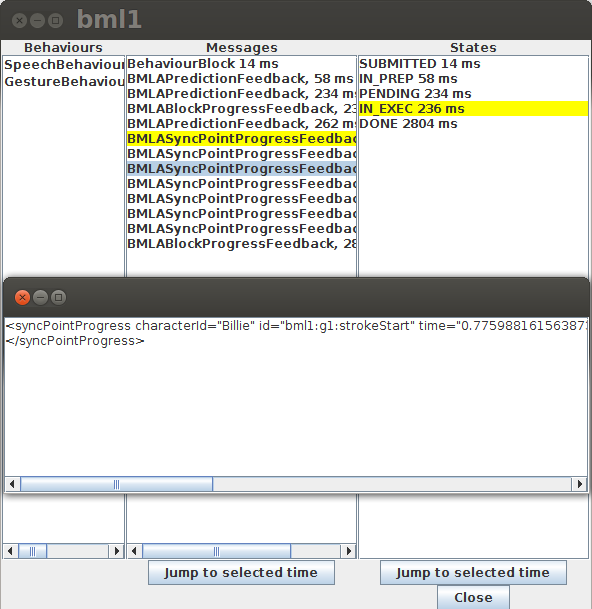
\includegraphics[width=0.9\textwidth]{images/bmlFlowBlockInfo.png}
 \caption{Block information window of the BMLFlowVisualizer. This gives detailed information about the different behaviours this block contained as well as the different received messages that are related to this block. The second window shows the textual information about a specific message.}
 \label{fig:info}
\end{figure}

\subsection{Block colours} \label{sec:colours}

As can already be seen in the example in figure \ref{fig:overview}, the blocks have different colours. The colours represent the current state of the bml blocks. A quick overview about the meaning of the different colours can be found in the Information window, accessible using the menu or the shortcut $CTRL+I$. Currently not all possible bml states have their own colour, mainly because not all possible states were actually used at this time.

Figure \ref{fig:help} shows the above mentioned Information window, including the meaning of the different colours

\begin{figure}[!htb]
\centering
 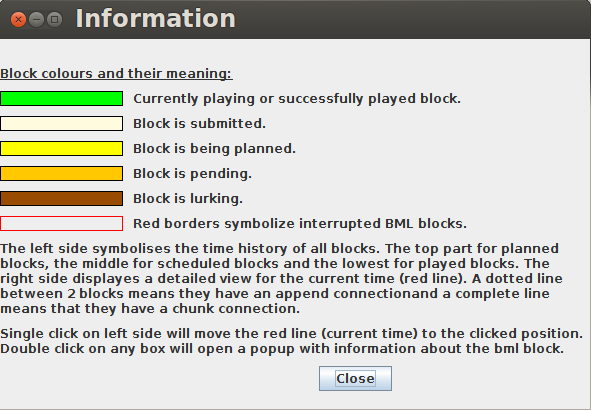
\includegraphics[width=0.9\textwidth]{images/bmlFlowInfo.png}
 \caption{General Information window of the BMLFlowVisualizer. This gives information about the different block colours as well as an overview about the program in general.}
 \label{fig:help}
\end{figure}


\section{Implementation Details}

In this section a few implementation details will be given.

\subsection{BMLBlocks}

A BML session always consist out of at least one bml block that is processed and goes through several phases. Information about the phases is being published to registered listeners by events (see section \ref{sec:eventflow} for details). In the BMLFlowVisualizer all the received information about a given bml block is stored in an object call BMLBlock. The information this class stores include all the feedback messages that were received concerning the block and information about the bml block status including the times these statuses were updated. Furthermore the BMLBlock class provides helper functions for other functionality of the program like formatting the included behaviours.

\subsection{Event flow} \label{sec:eventflow}

The general concept of the event flow can be seen in figure \ref{fig:eventflow}.
There are two types of events: bml\_block information and feedback. Both these events are listened two by two separate listeners. In both cases the event message that is received is stored in a wrapper object called BMLInformation for saving (see \ref{sec:saveload} for more details). Afterwards, the event is processed which differs depending on the event type. \\

bml\_block: A bml\_block message is fairly simple. When receiving such an event. It is checked if the behaviour block contains the \textit{REPLACE} composition. In that case, the list of stored bmlBlocks is cleared since this signals a session reset.

If the list of BMLBlocks does not contain a BMLBlock with the id of the received bml block than the block will be added to the list. This check is only necessary, because network timing might deliver a feedback before a bml\_block event is received. Usually the bml block should not be present before and will be added to the list. Furthermore, each received bml block is analysed for interrupt behaviours or attributes. If an interrupt is found, the targeted bml block will be interrupted, i.e. the interrupted flag will be set for that BMLBlock. \\

Feedback: There are several different types of feedback events. The types that are used at this point in time in the BMLFlowVisualizer are: BMLABlockProgressFeedback, BMLAPredictionFeedback, BMLWarningFeedback and BMLSyncPointProgressFeedback.
Regardless of the event type, the feedback message will be added to the responsible BMLBlock and the status of the BMLBlock will be updated according to the event message. \\

BMLABlockProgressFeedback is used to communicate the sates DONE and IN\_EXEC. \\

BMLAPredictionFeedback is used to communicate the states IN\_PREP, PENDING and LURKING. Furthermore, behaviour synchronisation points will be updated according to contained behaviour predictions. \\

BMLWarningFeedback and BMLSyncPointProgressFeedback are not used to communicate any bml state progression, but can contain further information about bml blocks. \\

These messages are just added to the feedback list of the responsible BMLBlock and can be viewed in the BML Information window.

\begin{figure}[!htb]
\centering
 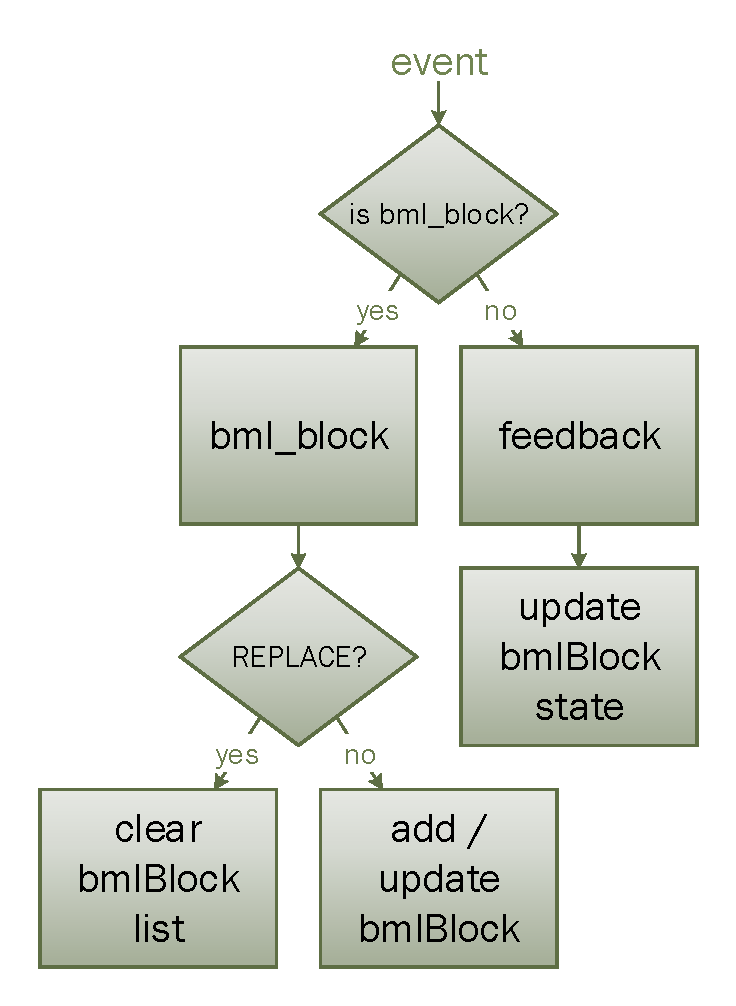
\includegraphics[width=0.5\textwidth]{images/bmlEventFlow.pdf}
 \caption{Overview about the event flow when receiving a bml message (either a bml\_block message or a feedback message).}
 \label{fig:eventflow}
\end{figure}

\subsection{Information about saving and loading a session} \label{sec:saveload}

The BMLFlowVisualizer can save a recorded session, which can be loaded and inspected at a later time. This is achieved by storing all the received feedback or bml blocks in a list of wrapper objects called BMLInformation. The BMLInformation stores the actual message, the type (feedback or bml\_block information) and the time the the message was received relative to the start of the first message that was received. When saving a session, the list of BMLInformation is serialized using standard Java serialisation and the resulting bytestring is stored in the given file. 


\end{document}